\let\negmedspace\undefined
\documentclass{beamer}
\mode<presentation>
\usepackage{amsmath}
\usepackage{amssymb}
%\usepackage{advdate}
\usepackage{adjustbox}
\usepackage{subcaption}
\usepackage{enumitem}
\usepackage{multicol}
\usepackage{mathtools}
\usepackage{listings}
\usepackage{url}
\def\UrlBreaks{\do\/\do-}
\usetheme{Madrid}
\usecolortheme{lily}
\setbeamertemplate{footline}
{
	\leavevmode%
	\hbox{%
		\begin{beamercolorbox}[wd=\paperwidth,ht=2.25ex,dp=1ex,right]{author in head/foot}%
			\insertframenumber{} / \inserttotalframenumber\hspace*{2ex} 
		\end{beamercolorbox}}%
		\vskip0pt%
	}
	\setbeamertemplate{navigation symbols}{}

	\providecommand{\nCr}[2]{\,^{#1}C_{#2}} % nCr
	\providecommand{\nPr}[2]{\,^{#1}P_{#2}} % nPr
	\providecommand{\mbf}{\mathbf}
	\providecommand{\pr}[1]{\ensuremath{\Pr\left(#1\right)}}
	\providecommand{\qfunc}[1]{\ensuremath{Q\left(#1\right)}}
	\providecommand{\sbrak}[1]{\ensuremath{{}\left[#1\right]}}
	\providecommand{\lsbrak}[1]{\ensuremath{{}\left[#1\right.}}
	\providecommand{\rsbrak}[1]{\ensuremath{{}\left.#1\right]}}
	\providecommand{\brak}[1]{\ensuremath{\left(#1\right)}}
	\providecommand{\lbrak}[1]{\ensuremath{\left(#1\right.}}
	\providecommand{\rbrak}[1]{\ensuremath{\left.#1\right)}}
	\providecommand{\cbrak}[1]{\ensuremath{\left\{#1\right\}}}
	\providecommand{\lcbrak}[1]{\ensuremath{\left\{#1\right.}}
	\providecommand{\rcbrak}[1]{\ensuremath{\left.#1\right\}}}
	\theoremstyle{remark}
	\newtheorem{rem}{Remark}
	\newcommand{\sgn}{\mathop{\mathrm{sgn}}}
	\providecommand{\abs}[1]{\left\vert#1\right\vert}
	\providecommand{\res}[1]{\Res\displaylimits_{#1}} 
	\providecommand{\norm}[1]{\lVert#1\rVert}
	\providecommand{\mtx}[1]{\mathbf{#1}}
	\providecommand{\mean}[1]{E\left[ #1 \right]}
	\providecommand{\fourier}{\overset{\mathcal{F}}{ \rightleftharpoons}}
	%\providecommand{\hilbert}{\overset{\mathcal{H}}{ \rightleftharpoons}}
	\providecommand{\system}{\overset{\mathcal{H}}{ \longleftrightarrow}}
	%\newcommand{\solution}[2]{\textbf{Solution:}{#1}}
	%\newcommand{\solution}{\noindent \textbf{Solution: }}
	\providecommand{\dec}[2]{\ensuremath{\overset{#1}{\underset{#2}{\gtrless}}}}
	\newcommand{\myvec}[1]{\ensuremath{\begin{pmatrix}#1\end{pmatrix}}}
		\let\vec\mathbf

		\lstset{
			%language=C,
			frame=single, 
			breaklines=true,
			columns=fullflexible
		}

		\numberwithin{equation}{section}

		\title{12.8.1.7}
		\author{EE24BTECH11018 - Durgi Swaraj Sharma}
		\date{}
		\begin{document}
		\frame{\titlepage}
		\begin{frame}
\textbf{6.6.13} Find the points at which the function $f$ given by $f\brak{x} = \brak{x-2}^4 \brak{x+1}^3$ has \brak{i} local maxima \brak{ii} local minima \brak{iii} point of inflection
		\end{frame}
		\begin{frame}
			\frametitle{\textbf{Theroretical solution}}
\begin{align}
	f\brak{x} &= \brak{x-2}^4\brak{x+1}^3\\
	f^{\prime}\brak{x} &= \brak{x-2}^3\brak{x+1}^2\brak{7x-2}
\end{align}
Setting $f^{\prime}\brak{x} = 0$, we get three critical points:
\begin{align}
	x &= 2\\ x &= -1\\ x &= \frac{2}{7}
\end{align}
		\end{frame}
		\begin{frame}
Checking the values of $f^{\prime}\brak{x}$ before and after these values of $x$, we can conclude that
\begin{align*}
	\text{there is a point of inflection at } x&=-1\\
	\text{there is a maxima at } x&=\frac{2}{7}\\
	\text{there is a minima at } x&=2
\end{align*}
		\end{frame}
		\begin{frame}
\textbf{Computational Solution}
This problem can be solved with the Gradient Descent algorithm.
The algorithm is implemented as
\begin{align}
	x_{n+1}&=x_n-\alpha f{\prime}\brak{x_n}\\
	x_{n+1}&=x_n-\alpha \brak{x+1}^2\brak{x-2}^4\brak{7x-2}
\end{align}
Where $\alpha$ is the learning rate. This algorithm is enough to find local minimum. The sign of $\alpha$ when set negative will change the algorithm to Gradient Ascent, which can be used to find local maximum.\\
We can find all the critial points and their nature by running the algorithm based on the currently acquired data.
		\end{frame}
		\begin{frame}
			\frametitle{Verification}
\begin{figure}
	\centering
	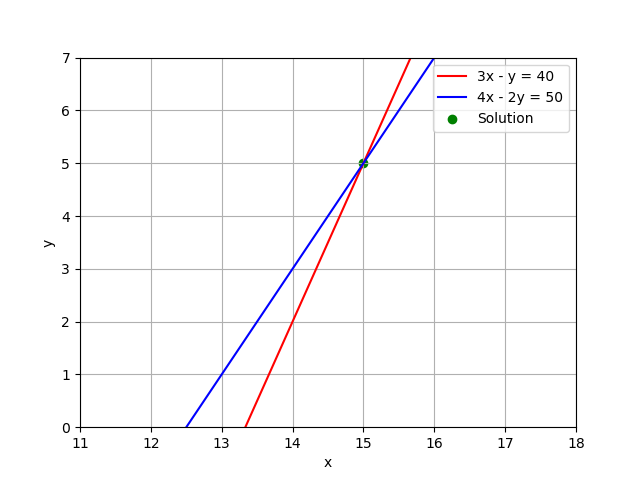
\includegraphics[width=0.8\columnwidth]{/home/gvt1/sdcard/github/EE1003/Assignment3/figs/fig.png}
	\caption{Demonstration}
\end{figure}
		\end{frame}
\end{document}
